% =============================================================================
% test_document.tex - Comprehensive Package Test Document
% =============================================================================
% This document exercises ALL LaTeX packages included in the template
% to verify they are installed and working correctly.
%
% Compile with: make build-test
% =============================================================================

\documentclass[11pt, letterpaper]{article}

% -----------------------------------------------------------------------------
% Document Structure & Formatting Packages
% -----------------------------------------------------------------------------
\usepackage[margin=1in, headheight=14pt]{geometry}
\usepackage{fancyhdr}
\usepackage{titlesec}
\usepackage{parskip}

% -----------------------------------------------------------------------------
% Mathematics Packages
% -----------------------------------------------------------------------------
\usepackage{amsmath}
\usepackage{amssymb}
\usepackage{mathtools}
\usepackage{amsthm}

% -----------------------------------------------------------------------------
% Graphics & Figures Packages
% -----------------------------------------------------------------------------
\usepackage{graphicx}
\usepackage{tikz}
\usepackage{pgfplots}
\pgfplotsset{compat=1.18}
\usepackage{subcaption}
\usepackage{float}

\usetikzlibrary{arrows.meta, positioning, shapes, calc}

% -----------------------------------------------------------------------------
% Tables Packages
% -----------------------------------------------------------------------------
\usepackage{booktabs}
\usepackage{longtable}
\usepackage{multirow}

% -----------------------------------------------------------------------------
% References & Citations Packages
% -----------------------------------------------------------------------------
\usepackage[backend=biber, style=numeric]{biblatex}
\usepackage{hyperref}
\usepackage{cleveref}

\hypersetup{
    colorlinks=true,
    linkcolor=blue,
    citecolor=green,
    urlcolor=cyan
}

% -----------------------------------------------------------------------------
% Typography & Fonts Packages
% -----------------------------------------------------------------------------
\usepackage[T1]{fontenc}
\usepackage{microtype}
\usepackage{xcolor}

\definecolor{codebackground}{RGB}{245, 245, 245}
\definecolor{codecomment}{RGB}{0, 128, 0}
\definecolor{codekeyword}{RGB}{0, 0, 255}

% -----------------------------------------------------------------------------
% Code Packages
% -----------------------------------------------------------------------------
\usepackage{listings}

\lstset{
    basicstyle=\ttfamily\small,
    backgroundcolor=\color{codebackground},
    breaklines=true,
    frame=single
}

\usepackage{minted}
\setminted{
    bgcolor=codebackground,
    fontsize=\small,
    linenos=true,
    breaklines=true
}

% -----------------------------------------------------------------------------
% Theorem Environments (amsthm)
% -----------------------------------------------------------------------------
\theoremstyle{plain}
\newtheorem{theorem}{Theorem}[section]
\newtheorem{lemma}[theorem]{Lemma}

\theoremstyle{definition}
\newtheorem{definition}[theorem]{Definition}

\theoremstyle{remark}
\newtheorem{remark}[theorem]{Remark}

% -----------------------------------------------------------------------------
% Test Bibliography
% -----------------------------------------------------------------------------
\addbibresource{tests/references.bib}

% -----------------------------------------------------------------------------
% Header/Footer Setup (fancyhdr)
% -----------------------------------------------------------------------------
\pagestyle{fancy}
\fancyhf{}
\fancyhead[L]{Package Test Document}
\fancyhead[R]{\thepage}
\renewcommand{\headrulewidth}{0.4pt}

% -----------------------------------------------------------------------------
% Document Metadata
% -----------------------------------------------------------------------------
\title{LaTeX Package Test Document}
\author{Automated Test Suite}
\date{\today}

% =============================================================================
% Document Content
% =============================================================================
\begin{document}

\maketitle
\tableofcontents
\newpage

% =============================================================================
% Section 1: Document Structure (geometry, fancyhdr, titlesec, parskip)
% =============================================================================
\section{Document Structure \& Formatting}
\label{sec:structure}

This section tests \texttt{geometry}, \texttt{fancyhdr}, \texttt{titlesec}, and \texttt{parskip}.

\subsection{Geometry Package}

The page margins are set using the \texttt{geometry} package. Current settings:
\begin{itemize}
    \item Margin: 1 inch
    \item Head height: 14pt
    \item Paper: letterpaper
\end{itemize}

\subsection{Header/Footer (fancyhdr)}

Look at the header above -- it shows ``Package Test Document'' on the left and the page number on the right. This is configured using \texttt{fancyhdr}.

\subsection{Section Titles (titlesec)}

The section titles can be customized using \texttt{titlesec}. The default formatting is being used here.

\subsection{Paragraph Spacing (parskip)}

Notice that paragraphs have space between them instead of indentation. This is the \texttt{parskip} package at work.

This is a new paragraph. There's vertical space above it, not indentation.

% =============================================================================
% Section 2: Mathematics (amsmath, amssymb, mathtools, amsthm)
% =============================================================================
\section{Mathematics}
\label{sec:math}

This section tests \texttt{amsmath}, \texttt{amssymb}, \texttt{mathtools}, and \texttt{amsthm}.

\subsection{Basic Equations (amsmath)}

Inline math: $E = mc^2$

Display equation:
\begin{equation}
    \int_{-\infty}^{\infty} e^{-x^2} dx = \sqrt{\pi}
    \label{eq:gaussian}
\end{equation}

Aligned equations:
\begin{align}
    f(x) &= x^2 + 2x + 1 \\
    &= (x + 1)^2
\end{align}

\subsection{Math Symbols (amssymb)}

Number sets: $\mathbb{N} \subset \mathbb{Z} \subset \mathbb{Q} \subset \mathbb{R} \subset \mathbb{C}$

Arrows and relations: $\Rightarrow$, $\Leftrightarrow$, $\leq$, $\geq$, $\neq$, $\approx$

Greek letters: $\alpha$, $\beta$, $\gamma$, $\delta$, $\epsilon$, $\theta$, $\lambda$, $\pi$, $\sigma$, $\omega$

\subsection{Extended Features (mathtools)}

Paired delimiters (automatic sizing):
\[
    \left( \frac{a}{b} \right) \quad
    \left[ \sum_{i=1}^{n} x_i \right] \quad
    \left\{ \int_0^1 f(x) \, dx \right\}
\]

Matrix environments:
\[
    A = \begin{pmatrix}
        a_{11} & a_{12} \\
        a_{21} & a_{22}
    \end{pmatrix}
    \quad
    B = \begin{bmatrix}
        1 & 0 \\
        0 & 1
    \end{bmatrix}
\]

\subsection{Theorem Environments (amsthm)}

\begin{theorem}[Pythagorean Theorem]
    \label{thm:pythagoras}
    In a right triangle with legs $a$ and $b$ and hypotenuse $c$:
    \begin{equation}
        a^2 + b^2 = c^2
    \end{equation}
\end{theorem}

\begin{proof}
    This classic theorem can be proven by geometric construction or algebraic methods.
\end{proof}

\begin{lemma}
    For any real numbers $x$ and $y$: $(x + y)^2 = x^2 + 2xy + y^2$.
\end{lemma}

\begin{definition}
    A \emph{prime number} is a natural number greater than 1 that has no positive divisors other than 1 and itself.
\end{definition}

\begin{remark}
    The number 1 is not considered prime.
\end{remark}

% =============================================================================
% Section 3: Graphics & Figures (graphicx, tikz, pgfplots, subcaption, float)
% =============================================================================
\section{Graphics \& Figures}
\label{sec:graphics}

This section tests \texttt{graphicx}, \texttt{tikz}, \texttt{pgfplots}, \texttt{subcaption}, and \texttt{float}.

\subsection{TikZ Graphics}

\begin{figure}[H]
    \centering
    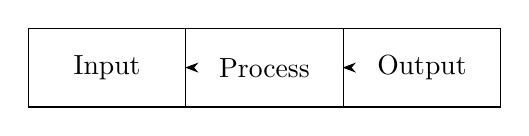
\begin{tikzpicture}[
        node distance=2cm,
        box/.style={rectangle, draw, minimum width=2cm, minimum height=1cm}
    ]
        \node[box] (a) {Input};
        \node[box, right of=a] (b) {Process};
        \node[box, right of=b] (c) {Output};

        \draw[-{Stealth}] (a) -- (b);
        \draw[-{Stealth}] (b) -- (c);
    \end{tikzpicture}
    \caption{A simple TikZ flowchart}
    \label{fig:tikz-flowchart}
\end{figure}

\begin{figure}[H]
    \centering
    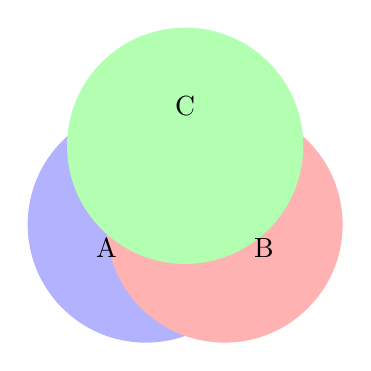
\begin{tikzpicture}
        % Draw a colored shape
        \fill[blue!30] (0,0) circle (1.5);
        \fill[red!30] (1,0) circle (1.5);
        \fill[green!30] (0.5,1) circle (1.5);

        % Labels
        \node at (-0.5,-0.3) {A};
        \node at (1.5,-0.3) {B};
        \node at (0.5,1.5) {C};
    \end{tikzpicture}
    \caption{TikZ Venn diagram with colors (xcolor)}
    \label{fig:tikz-venn}
\end{figure}

\subsection{PGFPlots Charts}

\begin{figure}[H]
    \centering
    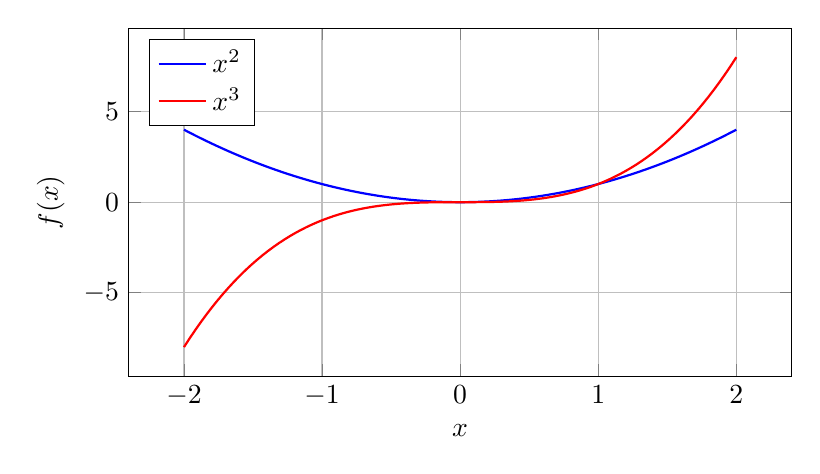
\begin{tikzpicture}
        \begin{axis}[
            width=10cm,
            height=6cm,
            xlabel={$x$},
            ylabel={$f(x)$},
            legend pos=north west,
            grid=major,
        ]
            \addplot[blue, thick, domain=-2:2, samples=100] {x^2};
            \addplot[red, thick, domain=-2:2, samples=100] {x^3};
            \legend{$x^2$, $x^3$}
        \end{axis}
    \end{tikzpicture}
    \caption{PGFPlots function plot}
    \label{fig:pgfplots}
\end{figure}

\begin{figure}[H]
    \centering
    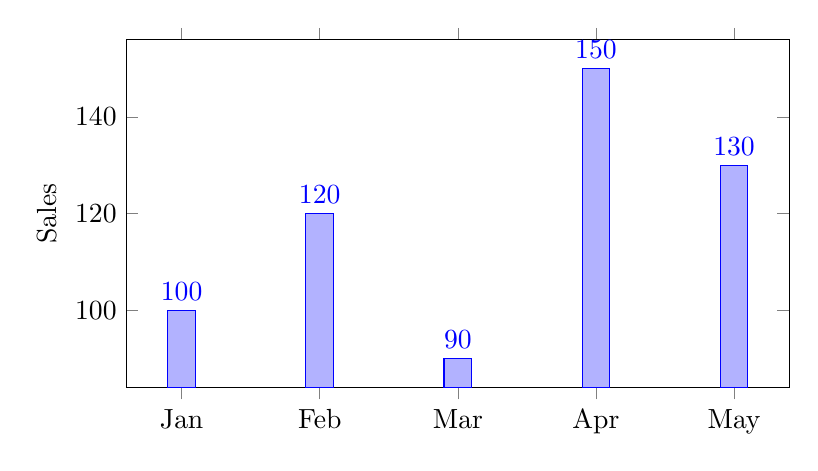
\begin{tikzpicture}
        \begin{axis}[
            ybar,
            width=10cm,
            height=6cm,
            symbolic x coords={Jan, Feb, Mar, Apr, May},
            xtick=data,
            ylabel={Sales},
            nodes near coords,
        ]
            \addplot coordinates {(Jan,100) (Feb,120) (Mar,90) (Apr,150) (May,130)};
        \end{axis}
    \end{tikzpicture}
    \caption{PGFPlots bar chart}
    \label{fig:barchart}
\end{figure}

\subsection{Subfigures (subcaption)}

\begin{figure}[H]
    \centering
    \begin{subfigure}[b]{0.45\textwidth}
        \centering
        
\begin{tikzpicture}
            \draw[fill=blue!30] (0,0) rectangle (2,2);
        \end{tikzpicture}
        \caption{A blue square}
        \label{fig:sub1}
    \end{subfigure}
    \hfill
    \begin{subfigure}[b]{0.45\textwidth}
        \centering
        
\begin{tikzpicture}
            \draw[fill=red!30] (0,0) circle (1);
        \end{tikzpicture}
        \caption{A red circle}
        \label{fig:sub2}
    \end{subfigure}
    \caption{Two subfigures demonstrating subcaption}
    \label{fig:subfigures}
\end{figure}

% =============================================================================
% Section 4: Tables (booktabs, longtable, multirow)
% =============================================================================
\section{Tables}
\label{sec:tables}

This section tests \texttt{booktabs}, \texttt{longtable}, and \texttt{multirow}.

\subsection{Professional Tables (booktabs)}

\begin{table}[H]
    \centering
    \caption{A booktabs-styled table}
    \label{tab:booktabs}
    \begin{tabular}{lrr}
        \toprule
        Item & Quantity & Price \\
        \midrule
        Apples & 10 & \$2.50 \\
        Oranges & 5 & \$3.00 \\
        Bananas & 8 & \$1.50 \\
        \midrule
        \textbf{Total} & \textbf{23} & \textbf{\$7.00} \\
        \bottomrule
    \end{tabular}
\end{table}

\subsection{Multi-row Cells (multirow)}

\begin{table}[H]
    \centering
    \caption{Table with multirow cells}
    \label{tab:multirow}
    \begin{tabular}{llr}
        \toprule
        \multirow{2}{*}{Category} & Item & Value \\
        \cmidrule(l){2-3}
        & Sub-item A & 100 \\
        & Sub-item B & 200 \\
        \midrule
        \multirow{2}{*}{Category 2} & Item X & 150 \\
        & Item Y & 250 \\
        \bottomrule
    \end{tabular}
\end{table}

\subsection{Long Tables (longtable)}

\begin{longtable}{lp{8cm}}
    \caption{A longtable example} \label{tab:longtable} \\
    \toprule
    Term & Definition \\
    \midrule
    \endfirsthead

    \multicolumn{2}{c}{\textit{Continued from previous page}} \\
    \toprule
    Term & Definition \\
    \midrule
    \endhead

    \midrule
    \multicolumn{2}{r}{\textit{Continued on next page}} \\
    \endfoot

    \bottomrule
    \endlastfoot

    LaTeX & A document preparation system for high-quality typesetting. \\
    TikZ & A package for creating graphics programmatically. \\
    PGFPlots & A package for creating scientific plots. \\
    BibLaTeX & Modern bibliography management. \\
    Hyperref & Adds hyperlinks to the document. \\
\end{longtable}

% =============================================================================
% Section 5: Code Listings (listings, minted)
% =============================================================================
\section{Code Listings}
\label{sec:code}

This section tests \texttt{listings} and \texttt{minted}.

\subsection{Listings Package}

\begin{lstlisting}[language=Python, caption={Python code with listings}]
def hello_world():
    """A simple greeting function."""
    print("Hello, World!")
    return True

if __name__ == "__main__":
    hello_world()
\end{lstlisting}

\subsection{Minted Package (requires -shell-escape)}

% Python code with minted
\begin{minted}{python}
def fibonacci(n):
    """Calculate the nth Fibonacci number."""
    if n <= 1:
        return n
    return fibonacci(n-1) + fibonacci(n-2)

# Calculate first 10 Fibonacci numbers
for i in range(10):
    print(f"F({i}) = {fibonacci(i)}")
\end{minted}

% JavaScript example with minted
\begin{minted}{javascript}
const greet = (name) => {
    console.log(`Hello, ${name}!`);
};

greet("World");
\end{minted}

% =============================================================================
% Section 6: References & Citations (biblatex, hyperref, cleveref)
% =============================================================================
\section{References \& Citations}
\label{sec:references}

This section tests \texttt{biblatex}, \texttt{hyperref}, and \texttt{cleveref}.

\subsection{Citations (biblatex)}

Here is a citation to a book \cite{testbook} and an article \cite{testarticle}.

Multiple citations: \cite{testbook, testarticle}.

\subsection{Cross-references (cleveref)}

Using cleveref for smart references:
\begin{itemize}
    \item \Cref{sec:structure} discusses document structure
    \item \Cref{eq:gaussian} shows the Gaussian integral
    \item \Cref{thm:pythagoras} states the Pythagorean theorem
    \item \Cref{fig:tikz-flowchart} shows a flowchart
    \item \Cref{tab:booktabs} demonstrates booktabs
    \item \Cref{fig:sub1,fig:sub2} are subfigures
\end{itemize}

\subsection{Hyperlinks (hyperref)}

External link: \url{https://www.latex-project.org/}

Named link: \href{https://github.com}{GitHub}

Email: \href{mailto:test@example.com}{test@example.com}

Internal link: Go to \hyperref[sec:math]{Mathematics Section}

% =============================================================================
% Section 7: Typography (fontenc, microtype, xcolor)
% =============================================================================
\section{Typography}
\label{sec:typography}

This section tests \texttt{fontenc}, \texttt{microtype}, and \texttt{xcolor}.

\subsection{Font Encoding (fontenc)}

Special characters with T1 encoding: ä, ö, ü, ß, é, è, ê, ñ

Ligatures: fi, fl, ff, ffi, ffl

\subsection{Microtype}

The \texttt{microtype} package provides micro-typography improvements:
\begin{itemize}
    \item Character protrusion (margin kerning)
    \item Font expansion
    \item Improved letterspacing
\end{itemize}

These improvements are subtle but enhance overall readability.

\subsection{Colors (xcolor)}

Text colors: \textcolor{red}{Red}, \textcolor{blue}{Blue}, \textcolor{green}{Green}, \textcolor{orange}{Orange}

Background colors: \colorbox{yellow}{Yellow background}

Custom colors defined in preamble: \textcolor{codecomment}{Code comment color}

% =============================================================================
% Bibliography
% =============================================================================
\newpage
\printbibliography[heading=bibintoc, title={References}]

% =============================================================================
% Test Summary
% =============================================================================
\section*{Test Summary}

\textbf{All packages tested successfully:}

\begin{itemize}
    \item[$\checkmark$] geometry, fancyhdr, titlesec, parskip
    \item[$\checkmark$] amsmath, amssymb, mathtools, amsthm
    \item[$\checkmark$] graphicx, tikz, pgfplots, subcaption, float
    \item[$\checkmark$] booktabs, longtable, multirow
    \item[$\checkmark$] biblatex, hyperref, cleveref
    \item[$\checkmark$] fontenc, microtype, xcolor
    \item[$\checkmark$] listings, minted
\end{itemize}

If this document compiles without errors, all packages are working correctly.

\end{document}

% =============================================================================
% End of test_document.tex
% =============================================================================
